% Created by tikzDevice version 0.12.6 on 2026-03-17 20:30:56
% !TEX encoding = UTF-8 Unicode
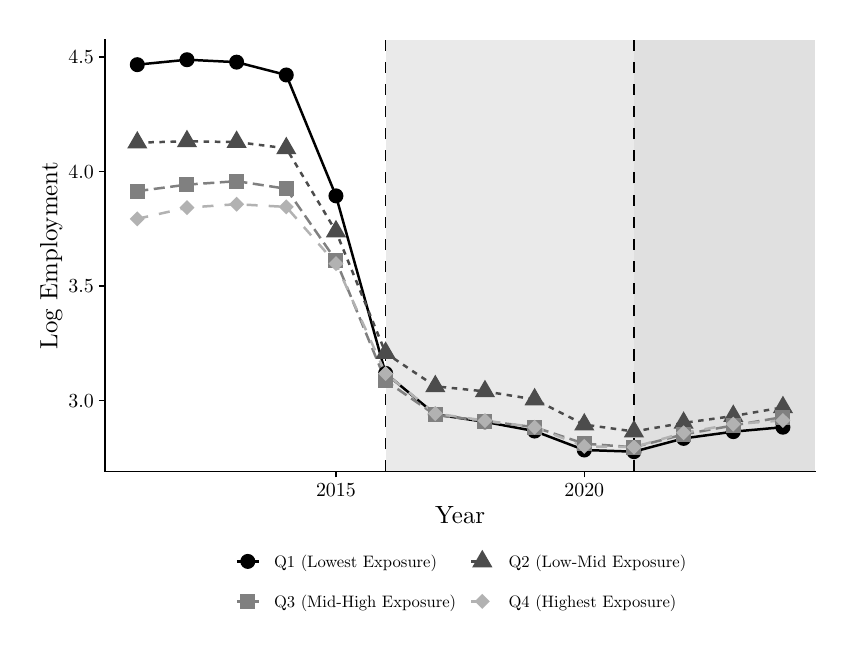
\begin{tikzpicture}[x=1pt,y=1pt]
\definecolor{fillColor}{RGB}{255,255,255}
\path[use as bounding box,fill=fillColor,fill opacity=0.00] (0,0) rectangle (289.08,216.81);
\begin{scope}
\path[clip] (  0.00,  0.00) rectangle (289.08,216.81);
\definecolor{drawColor}{RGB}{255,255,255}
\definecolor{fillColor}{RGB}{255,255,255}

\path[draw=drawColor,line width= 0.5pt,line join=round,line cap=round,fill=fillColor] (  0.00,  0.00) rectangle (289.08,216.81);
\end{scope}
\begin{scope}
\path[clip] ( 27.95, 56.52) rectangle (284.58,212.31);
\definecolor{fillColor}{RGB}{255,255,255}

\path[fill=fillColor] ( 27.95, 56.52) rectangle (284.58,212.31);
\definecolor{fillColor}{RGB}{153,153,153}

\path[fill=fillColor,fill opacity=0.20] (129.34, 56.52) rectangle (219.08,212.31);
\definecolor{fillColor}{RGB}{102,102,102}

\path[fill=fillColor,fill opacity=0.20] (219.08, 56.52) rectangle (284.58,212.31);
\definecolor{drawColor}{RGB}{0,0,0}

\path[draw=drawColor,line width= 0.6pt,dash pattern=on 4pt off 4pt ,line join=round] (129.34, 56.52) -- (129.34,212.31);

\path[draw=drawColor,line width= 0.6pt,dash pattern=on 4pt off 4pt ,line join=round] (219.08, 56.52) -- (219.08,212.31);

\path[draw=drawColor,line width= 0.9pt,line join=round] ( 39.61,203.44) --
	( 57.56,205.23) --
	( 75.50,204.35) --
	( 93.45,199.71) --
	(111.40,156.03) --
	(129.34, 91.88) --
	(147.29, 77.07) --
	(165.24, 74.37) --
	(183.18, 71.04) --
	(201.13, 64.20) --
	(219.08, 63.60) --
	(237.02, 68.39) --
	(254.97, 70.83) --
	(272.91, 72.44);
\definecolor{drawColor}{gray}{0.30}

\path[draw=drawColor,line width= 0.9pt,dash pattern=on 2pt off 2pt ,line join=round] ( 39.61,175.27) --
	( 57.56,175.73) --
	( 75.50,175.49) --
	( 93.45,173.21) --
	(111.40,143.18) --
	(129.34, 99.27) --
	(147.29, 87.21) --
	(165.24, 85.39) --
	(183.18, 82.48) --
	(201.13, 73.38) --
	(219.08, 70.89) --
	(237.02, 74.00) --
	(254.97, 76.47) --
	(272.91, 79.61);
\definecolor{drawColor}{gray}{0.50}

\path[draw=drawColor,line width= 0.9pt,dash pattern=on 4pt off 2pt ,line join=round] ( 39.61,157.74) --
	( 57.56,160.09) --
	( 75.50,161.34) --
	( 93.45,158.60) --
	(111.40,132.71) --
	(129.34, 89.22) --
	(147.29, 76.86) --
	(165.24, 74.66) --
	(183.18, 72.44) --
	(201.13, 66.49) --
	(219.08, 65.20) --
	(237.02, 69.84) --
	(254.97, 73.07) --
	(272.91, 76.11);
\definecolor{drawColor}{gray}{0.70}

\path[draw=drawColor,line width= 0.9pt,dash pattern=on 4pt off 4pt ,line join=round] ( 39.61,147.73) --
	( 57.56,151.77) --
	( 75.50,153.02) --
	( 93.45,152.04) --
	(111.40,131.53) --
	(129.34, 91.81) --
	(147.29, 77.38) --
	(165.24, 74.82) --
	(183.18, 72.46) --
	(201.13, 65.51) --
	(219.08, 65.24) --
	(237.02, 70.40) --
	(254.97, 73.55) --
	(272.91, 74.88);
\definecolor{fillColor}{RGB}{0,0,0}

\path[fill=fillColor] ( 39.61,203.44) circle (  2.71);
\definecolor{fillColor}{gray}{0.30}

\path[fill=fillColor] ( 39.61,179.49) --
	( 43.26,173.16) --
	( 35.96,173.16) --
	cycle;
\definecolor{fillColor}{gray}{0.50}

\path[fill=fillColor] ( 36.90,155.03) --
	( 42.32,155.03) --
	( 42.32,160.46) --
	( 36.90,160.46) --
	cycle;
\definecolor{fillColor}{gray}{0.70}

\path[fill=fillColor] ( 36.90,147.73) --
	( 39.61,150.44) --
	( 42.32,147.73) --
	( 39.61,145.02) --
	cycle;
\definecolor{fillColor}{RGB}{0,0,0}

\path[fill=fillColor] ( 57.56,205.23) circle (  2.71);
\definecolor{fillColor}{gray}{0.30}

\path[fill=fillColor] ( 57.56,179.95) --
	( 61.21,173.62) --
	( 53.91,173.62) --
	cycle;
\definecolor{fillColor}{gray}{0.50}

\path[fill=fillColor] ( 54.85,157.38) --
	( 60.27,157.38) --
	( 60.27,162.81) --
	( 54.85,162.81) --
	cycle;
\definecolor{fillColor}{gray}{0.70}

\path[fill=fillColor] ( 54.85,151.77) --
	( 57.56,154.49) --
	( 60.27,151.77) --
	( 57.56,149.06) --
	cycle;
\definecolor{fillColor}{RGB}{0,0,0}

\path[fill=fillColor] ( 75.50,204.35) circle (  2.71);
\definecolor{fillColor}{gray}{0.30}

\path[fill=fillColor] ( 75.50,179.71) --
	( 79.15,173.38) --
	( 71.85,173.38) --
	cycle;
\definecolor{fillColor}{gray}{0.50}

\path[fill=fillColor] ( 72.79,158.63) --
	( 78.21,158.63) --
	( 78.21,164.05) --
	( 72.79,164.05) --
	cycle;
\definecolor{fillColor}{gray}{0.70}

\path[fill=fillColor] ( 72.79,153.02) --
	( 75.50,155.73) --
	( 78.21,153.02) --
	( 75.50,150.30) --
	cycle;
\definecolor{fillColor}{RGB}{0,0,0}

\path[fill=fillColor] ( 93.45,199.71) circle (  2.71);
\definecolor{fillColor}{gray}{0.30}

\path[fill=fillColor] ( 93.45,177.42) --
	( 97.10,171.10) --
	( 89.80,171.10) --
	cycle;
\definecolor{fillColor}{gray}{0.50}

\path[fill=fillColor] ( 90.74,155.89) --
	( 96.16,155.89) --
	( 96.16,161.31) --
	( 90.74,161.31) --
	cycle;
\definecolor{fillColor}{gray}{0.70}

\path[fill=fillColor] ( 90.74,152.04) --
	( 93.45,154.75) --
	( 96.16,152.04) --
	( 93.45,149.33) --
	cycle;
\definecolor{fillColor}{RGB}{0,0,0}

\path[fill=fillColor] (111.40,156.03) circle (  2.71);
\definecolor{fillColor}{gray}{0.30}

\path[fill=fillColor] (111.40,147.39) --
	(115.05,141.07) --
	(107.75,141.07) --
	cycle;
\definecolor{fillColor}{gray}{0.50}

\path[fill=fillColor] (108.69,130.00) --
	(114.11,130.00) --
	(114.11,135.42) --
	(108.69,135.42) --
	cycle;
\definecolor{fillColor}{gray}{0.70}

\path[fill=fillColor] (108.69,131.53) --
	(111.40,134.25) --
	(114.11,131.53) --
	(111.40,128.82) --
	cycle;
\definecolor{fillColor}{RGB}{0,0,0}

\path[fill=fillColor] (129.34, 91.88) circle (  2.71);
\definecolor{fillColor}{gray}{0.30}

\path[fill=fillColor] (129.34,103.48) --
	(132.99, 97.16) --
	(125.69, 97.16) --
	cycle;
\definecolor{fillColor}{gray}{0.50}

\path[fill=fillColor] (126.63, 86.51) --
	(132.05, 86.51) --
	(132.05, 91.93) --
	(126.63, 91.93) --
	cycle;
\definecolor{fillColor}{gray}{0.70}

\path[fill=fillColor] (126.63, 91.81) --
	(129.34, 94.52) --
	(132.05, 91.81) --
	(129.34, 89.10) --
	cycle;
\definecolor{fillColor}{RGB}{0,0,0}

\path[fill=fillColor] (147.29, 77.07) circle (  2.71);
\definecolor{fillColor}{gray}{0.30}

\path[fill=fillColor] (147.29, 91.42) --
	(150.94, 85.10) --
	(143.64, 85.10) --
	cycle;
\definecolor{fillColor}{gray}{0.50}

\path[fill=fillColor] (144.58, 74.15) --
	(150.00, 74.15) --
	(150.00, 79.57) --
	(144.58, 79.57) --
	cycle;
\definecolor{fillColor}{gray}{0.70}

\path[fill=fillColor] (144.58, 77.38) --
	(147.29, 80.09) --
	(150.00, 77.38) --
	(147.29, 74.66) --
	cycle;
\definecolor{fillColor}{RGB}{0,0,0}

\path[fill=fillColor] (165.24, 74.37) circle (  2.71);
\definecolor{fillColor}{gray}{0.30}

\path[fill=fillColor] (165.24, 89.60) --
	(168.89, 83.28) --
	(161.58, 83.28) --
	cycle;
\definecolor{fillColor}{gray}{0.50}

\path[fill=fillColor] (162.53, 71.95) --
	(167.95, 71.95) --
	(167.95, 77.37) --
	(162.53, 77.37) --
	cycle;
\definecolor{fillColor}{gray}{0.70}

\path[fill=fillColor] (162.53, 74.82) --
	(165.24, 77.53) --
	(167.95, 74.82) --
	(165.24, 72.11) --
	cycle;
\definecolor{fillColor}{RGB}{0,0,0}

\path[fill=fillColor] (183.18, 71.04) circle (  2.71);
\definecolor{fillColor}{gray}{0.30}

\path[fill=fillColor] (183.18, 86.69) --
	(186.83, 80.37) --
	(179.53, 80.37) --
	cycle;
\definecolor{fillColor}{gray}{0.50}

\path[fill=fillColor] (180.47, 69.73) --
	(185.89, 69.73) --
	(185.89, 75.15) --
	(180.47, 75.15) --
	cycle;
\definecolor{fillColor}{gray}{0.70}

\path[fill=fillColor] (180.47, 72.46) --
	(183.18, 75.17) --
	(185.89, 72.46) --
	(183.18, 69.75) --
	cycle;
\definecolor{fillColor}{RGB}{0,0,0}

\path[fill=fillColor] (201.13, 64.20) circle (  2.71);
\definecolor{fillColor}{gray}{0.30}

\path[fill=fillColor] (201.13, 77.60) --
	(204.78, 71.27) --
	(197.48, 71.27) --
	cycle;
\definecolor{fillColor}{gray}{0.50}

\path[fill=fillColor] (198.42, 63.78) --
	(203.84, 63.78) --
	(203.84, 69.20) --
	(198.42, 69.20) --
	cycle;
\definecolor{fillColor}{gray}{0.70}

\path[fill=fillColor] (198.42, 65.51) --
	(201.13, 68.23) --
	(203.84, 65.51) --
	(201.13, 62.80) --
	cycle;
\definecolor{fillColor}{RGB}{0,0,0}

\path[fill=fillColor] (219.08, 63.60) circle (  2.71);
\definecolor{fillColor}{gray}{0.30}

\path[fill=fillColor] (219.08, 75.11) --
	(222.73, 68.78) --
	(215.42, 68.78) --
	cycle;
\definecolor{fillColor}{gray}{0.50}

\path[fill=fillColor] (216.36, 62.49) --
	(221.79, 62.49) --
	(221.79, 67.92) --
	(216.36, 67.92) --
	cycle;
\definecolor{fillColor}{gray}{0.70}

\path[fill=fillColor] (216.36, 65.24) --
	(219.08, 67.95) --
	(221.79, 65.24) --
	(219.08, 62.53) --
	cycle;
\definecolor{fillColor}{RGB}{0,0,0}

\path[fill=fillColor] (237.02, 68.39) circle (  2.71);
\definecolor{fillColor}{gray}{0.30}

\path[fill=fillColor] (237.02, 78.21) --
	(240.67, 71.89) --
	(233.37, 71.89) --
	cycle;
\definecolor{fillColor}{gray}{0.50}

\path[fill=fillColor] (234.31, 67.13) --
	(239.73, 67.13) --
	(239.73, 72.55) --
	(234.31, 72.55) --
	cycle;
\definecolor{fillColor}{gray}{0.70}

\path[fill=fillColor] (234.31, 70.40) --
	(237.02, 73.11) --
	(239.73, 70.40) --
	(237.02, 67.69) --
	cycle;
\definecolor{fillColor}{RGB}{0,0,0}

\path[fill=fillColor] (254.97, 70.83) circle (  2.71);
\definecolor{fillColor}{gray}{0.30}

\path[fill=fillColor] (254.97, 80.69) --
	(258.62, 74.36) --
	(251.32, 74.36) --
	cycle;
\definecolor{fillColor}{gray}{0.50}

\path[fill=fillColor] (252.26, 70.36) --
	(257.68, 70.36) --
	(257.68, 75.78) --
	(252.26, 75.78) --
	cycle;
\definecolor{fillColor}{gray}{0.70}

\path[fill=fillColor] (252.26, 73.55) --
	(254.97, 76.26) --
	(257.68, 73.55) --
	(254.97, 70.84) --
	cycle;
\definecolor{fillColor}{RGB}{0,0,0}

\path[fill=fillColor] (272.91, 72.44) circle (  2.71);
\definecolor{fillColor}{gray}{0.30}

\path[fill=fillColor] (272.91, 83.82) --
	(276.57, 77.50) --
	(269.26, 77.50) --
	cycle;
\definecolor{fillColor}{gray}{0.50}

\path[fill=fillColor] (270.20, 73.40) --
	(275.63, 73.40) --
	(275.63, 78.82) --
	(270.20, 78.82) --
	cycle;
\definecolor{fillColor}{gray}{0.70}

\path[fill=fillColor] (270.20, 74.88) --
	(272.91, 77.59) --
	(275.63, 74.88) --
	(272.91, 72.17) --
	cycle;
\end{scope}
\begin{scope}
\path[clip] (  0.00,  0.00) rectangle (289.08,216.81);
\definecolor{drawColor}{RGB}{0,0,0}

\path[draw=drawColor,line width= 0.5pt,line join=round,line cap=rect] ( 27.95, 56.52) --
	( 27.95,212.31);
\end{scope}
\begin{scope}
\path[clip] (  0.00,  0.00) rectangle (289.08,216.81);
\definecolor{drawColor}{RGB}{0,0,0}

\node[text=drawColor,anchor=base east,inner sep=0pt, outer sep=0pt, scale=  0.72] at ( 23.90, 79.68) {3.0};

\node[text=drawColor,anchor=base east,inner sep=0pt, outer sep=0pt, scale=  0.72] at ( 23.90,121.05) {3.5};

\node[text=drawColor,anchor=base east,inner sep=0pt, outer sep=0pt, scale=  0.72] at ( 23.90,162.42) {4.0};

\node[text=drawColor,anchor=base east,inner sep=0pt, outer sep=0pt, scale=  0.72] at ( 23.90,203.78) {4.5};
\end{scope}
\begin{scope}
\path[clip] (  0.00,  0.00) rectangle (289.08,216.81);
\definecolor{drawColor}{RGB}{0,0,0}

\path[draw=drawColor,line width= 0.5pt,line join=round] ( 25.70, 82.16) --
	( 27.95, 82.16);

\path[draw=drawColor,line width= 0.5pt,line join=round] ( 25.70,123.53) --
	( 27.95,123.53);

\path[draw=drawColor,line width= 0.5pt,line join=round] ( 25.70,164.89) --
	( 27.95,164.89);

\path[draw=drawColor,line width= 0.5pt,line join=round] ( 25.70,206.26) --
	( 27.95,206.26);
\end{scope}
\begin{scope}
\path[clip] (  0.00,  0.00) rectangle (289.08,216.81);
\definecolor{drawColor}{RGB}{0,0,0}

\path[draw=drawColor,line width= 0.5pt,line join=round,line cap=rect] ( 27.95, 56.52) --
	(284.58, 56.52);
\end{scope}
\begin{scope}
\path[clip] (  0.00,  0.00) rectangle (289.08,216.81);
\definecolor{drawColor}{RGB}{0,0,0}

\path[draw=drawColor,line width= 0.5pt,line join=round] (111.40, 54.27) --
	(111.40, 56.52);

\path[draw=drawColor,line width= 0.5pt,line join=round] (201.13, 54.27) --
	(201.13, 56.52);
\end{scope}
\begin{scope}
\path[clip] (  0.00,  0.00) rectangle (289.08,216.81);
\definecolor{drawColor}{RGB}{0,0,0}

\node[text=drawColor,anchor=base,inner sep=0pt, outer sep=0pt, scale=  0.72] at (111.40, 47.51) {2015};

\node[text=drawColor,anchor=base,inner sep=0pt, outer sep=0pt, scale=  0.72] at (201.13, 47.51) {2020};
\end{scope}
\begin{scope}
\path[clip] (  0.00,  0.00) rectangle (289.08,216.81);
\definecolor{drawColor}{RGB}{0,0,0}

\node[text=drawColor,anchor=base,inner sep=0pt, outer sep=0pt, scale=  0.90] at (156.26, 37.67) {Year};
\end{scope}
\begin{scope}
\path[clip] (  0.00,  0.00) rectangle (289.08,216.81);
\definecolor{drawColor}{RGB}{0,0,0}

\node[text=drawColor,rotate= 90.00,anchor=base,inner sep=0pt, outer sep=0pt, scale=  0.90] at ( 10.70,134.42) {Log Employment};
\end{scope}
\begin{scope}
\path[clip] (  0.00,  0.00) rectangle (289.08,216.81);
\definecolor{drawColor}{RGB}{0,0,0}

\path[draw=drawColor,line width= 0.9pt,line join=round] ( 75.56, 23.94) -- ( 83.52, 23.94);
\definecolor{fillColor}{RGB}{0,0,0}

\path[fill=fillColor] ( 79.54, 23.94) circle (  2.71);
\end{scope}
\begin{scope}
\path[clip] (  0.00,  0.00) rectangle (289.08,216.81);
\definecolor{drawColor}{gray}{0.30}

\path[draw=drawColor,line width= 0.9pt,dash pattern=on 2pt off 2pt ,line join=round] (160.30, 23.94) -- (168.27, 23.94);
\definecolor{fillColor}{gray}{0.30}

\path[fill=fillColor] (164.28, 28.15) --
	(167.93, 21.83) --
	(160.63, 21.83) --
	cycle;
\end{scope}
\begin{scope}
\path[clip] (  0.00,  0.00) rectangle (289.08,216.81);
\definecolor{drawColor}{gray}{0.50}

\path[draw=drawColor,line width= 0.9pt,dash pattern=on 4pt off 2pt ,line join=round] ( 75.56,  9.48) -- ( 83.52,  9.48);
\definecolor{fillColor}{gray}{0.50}

\path[fill=fillColor] ( 76.83,  6.77) --
	( 82.25,  6.77) --
	( 82.25, 12.19) --
	( 76.83, 12.19) --
	cycle;
\end{scope}
\begin{scope}
\path[clip] (  0.00,  0.00) rectangle (289.08,216.81);
\definecolor{drawColor}{gray}{0.70}

\path[draw=drawColor,line width= 0.9pt,dash pattern=on 4pt off 4pt ,line join=round] (160.30,  9.48) -- (168.27,  9.48);
\definecolor{fillColor}{gray}{0.70}

\path[fill=fillColor] (161.57,  9.48) --
	(164.28, 12.19) --
	(166.99,  9.48) --
	(164.28,  6.77) --
	cycle;
\end{scope}
\begin{scope}
\path[clip] (  0.00,  0.00) rectangle (289.08,216.81);
\definecolor{drawColor}{RGB}{0,0,0}

\node[text=drawColor,anchor=base west,inner sep=0pt, outer sep=0pt, scale=  0.60] at ( 89.02, 21.87) {Q1 (Lowest Exposure)};
\end{scope}
\begin{scope}
\path[clip] (  0.00,  0.00) rectangle (289.08,216.81);
\definecolor{drawColor}{RGB}{0,0,0}

\node[text=drawColor,anchor=base west,inner sep=0pt, outer sep=0pt, scale=  0.60] at (173.76, 21.87) {Q2 (Low-Mid Exposure)};
\end{scope}
\begin{scope}
\path[clip] (  0.00,  0.00) rectangle (289.08,216.81);
\definecolor{drawColor}{RGB}{0,0,0}

\node[text=drawColor,anchor=base west,inner sep=0pt, outer sep=0pt, scale=  0.60] at ( 89.02,  7.41) {Q3 (Mid-High Exposure)};
\end{scope}
\begin{scope}
\path[clip] (  0.00,  0.00) rectangle (289.08,216.81);
\definecolor{drawColor}{RGB}{0,0,0}

\node[text=drawColor,anchor=base west,inner sep=0pt, outer sep=0pt, scale=  0.60] at (173.76,  7.41) {Q4 (Highest Exposure)};
\end{scope}
\end{tikzpicture}
